

\tikzset{every picture/.style={line width=0.75pt}} %set default line width to 0.75pt        

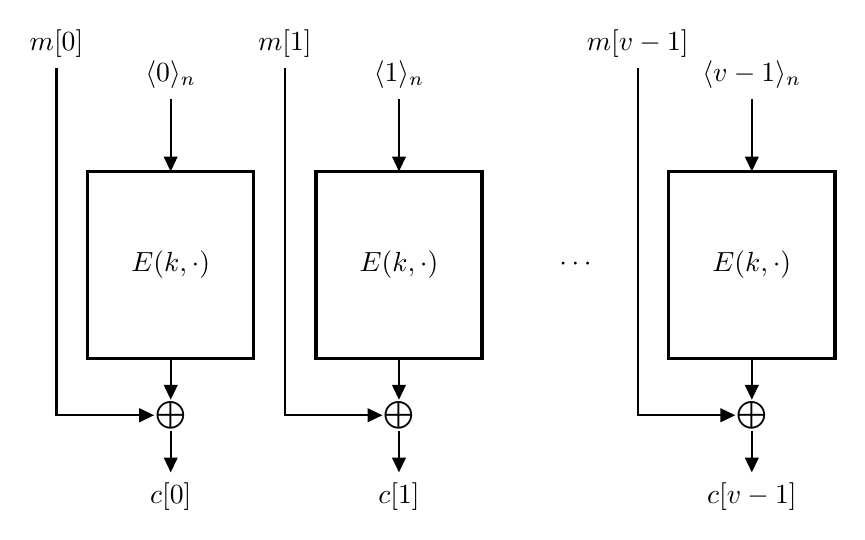
\begin{tikzpicture}[x=0.75pt,y=0.75pt,yscale=-1,xscale=1]
%uncomment if require: \path (0,278); %set diagram left start at 0, and has height of 278

%Shape: Rectangle [id:dp7999292839288346] 
\draw  [line width=1.2]  (30,80) -- (110,80) -- (110,170) -- (30,170) -- cycle ;
%Straight Lines [id:da21207260053300403] 
\draw    (70,45) -- (70,77) ;
\draw [shift={(70,80)}, rotate = 270] [fill={rgb, 255:red, 0; green, 0; blue, 0 }  ][line width=0.08]  [draw opacity=0] (7.14,-3.43) -- (0,0) -- (7.14,3.43) -- cycle    ;
%Straight Lines [id:da5786742487139955] 
\draw    (70.03,170) -- (70.03,187) ;
\draw [shift={(70.03,190)}, rotate = 270] [fill={rgb, 255:red, 0; green, 0; blue, 0 }  ][line width=0.08]  [draw opacity=0] (7.14,-3.43) -- (0,0) -- (7.14,3.43) -- cycle    ;
%Shape: Rectangle [id:dp33474182702855115] 
\draw  [line width=1.2]  (140,80) -- (220,80) -- (220,170) -- (140,170) -- cycle ;
%Straight Lines [id:da1941389963634068] 
\draw    (180,45) -- (180,77) ;
\draw [shift={(180,80)}, rotate = 270] [fill={rgb, 255:red, 0; green, 0; blue, 0 }  ][line width=0.08]  [draw opacity=0] (7.14,-3.43) -- (0,0) -- (7.14,3.43) -- cycle    ;
%Shape: Rectangle [id:dp37526129854437684] 
\draw  [line width=1.2]  (310,80) -- (390,80) -- (390,170) -- (310,170) -- cycle ;
%Straight Lines [id:da743177101791014] 
\draw    (350,45) -- (350,77) ;
\draw [shift={(350,80)}, rotate = 270] [fill={rgb, 255:red, 0; green, 0; blue, 0 }  ][line width=0.08]  [draw opacity=0] (7.14,-3.43) -- (0,0) -- (7.14,3.43) -- cycle    ;
%Straight Lines [id:da037465944110148364] 
\draw    (70.03,205) -- (70.03,222) ;
\draw [shift={(70.03,225)}, rotate = 270] [fill={rgb, 255:red, 0; green, 0; blue, 0 }  ][line width=0.08]  [draw opacity=0] (7.14,-3.43) -- (0,0) -- (7.14,3.43) -- cycle    ;
%Straight Lines [id:da25341296385169] 
\draw    (180,170) -- (180,187) ;
\draw [shift={(180,190)}, rotate = 270] [fill={rgb, 255:red, 0; green, 0; blue, 0 }  ][line width=0.08]  [draw opacity=0] (7.14,-3.43) -- (0,0) -- (7.14,3.43) -- cycle    ;
%Straight Lines [id:da549186584297201] 
\draw    (180,205) -- (180,222) ;
\draw [shift={(180,225)}, rotate = 270] [fill={rgb, 255:red, 0; green, 0; blue, 0 }  ][line width=0.08]  [draw opacity=0] (7.14,-3.43) -- (0,0) -- (7.14,3.43) -- cycle    ;
%Straight Lines [id:da1745260439609646] 
\draw    (350,170) -- (350,187) ;
\draw [shift={(350,190)}, rotate = 270] [fill={rgb, 255:red, 0; green, 0; blue, 0 }  ][line width=0.08]  [draw opacity=0] (7.14,-3.43) -- (0,0) -- (7.14,3.43) -- cycle    ;
%Straight Lines [id:da6402494560971277] 
\draw    (350,205) -- (350,222) ;
\draw [shift={(350,225)}, rotate = 270] [fill={rgb, 255:red, 0; green, 0; blue, 0 }  ][line width=0.08]  [draw opacity=0] (7.14,-3.43) -- (0,0) -- (7.14,3.43) -- cycle    ;
%Straight Lines [id:da5998735686530972] 
\draw    (15,30) -- (15,197.5) -- (59,197.5) ;
\draw [shift={(62,197.5)}, rotate = 180] [fill={rgb, 255:red, 0; green, 0; blue, 0 }  ][line width=0.08]  [draw opacity=0] (7.14,-3.43) -- (0,0) -- (7.14,3.43) -- cycle    ;
%Straight Lines [id:da43708262156487065] 
\draw    (125,30) -- (125,197.5) -- (169,197.5) ;
\draw [shift={(172,197.5)}, rotate = 180] [fill={rgb, 255:red, 0; green, 0; blue, 0 }  ][line width=0.08]  [draw opacity=0] (7.14,-3.43) -- (0,0) -- (7.14,3.43) -- cycle    ;
%Straight Lines [id:da39348763634018025] 
\draw    (295,30) -- (295,197.5) -- (339,197.5) ;
\draw [shift={(342,197.5)}, rotate = 180] [fill={rgb, 255:red, 0; green, 0; blue, 0 }  ][line width=0.08]  [draw opacity=0] (7.14,-3.43) -- (0,0) -- (7.14,3.43) -- cycle    ;

% Text Node
\draw (70,125) node    {$E( k,\cdot )$};
% Text Node
\draw (15,26.6) node [anchor=south] [inner sep=0.75pt]    {$m[ 0]$};
% Text Node
\draw (70.03,228.4) node [anchor=north] [inner sep=0.75pt]    {$c[ 0]$};
% Text Node
\draw (180,125) node    {$E( k,\cdot )$};
% Text Node
\draw (125,26.6) node [anchor=south] [inner sep=0.75pt]    {$m[ 1]$};
% Text Node
\draw (180,228.4) node [anchor=north] [inner sep=0.75pt]    {$c[ 1]$};
% Text Node
\draw (350,125) node    {$E( k,\cdot )$};
% Text Node
\draw (295,26.6) node [anchor=south] [inner sep=0.75pt]    {$m[ v-1]$};
% Text Node
\draw (350,228.4) node [anchor=north] [inner sep=0.75pt]    {$c[ v-1]$};
% Text Node
\draw (265,125) node    {$\cdots $};
% Text Node
\draw (70,197.5) node    {$\bigoplus $};
% Text Node
\draw (180,197.5) node    {$\bigoplus $};
% Text Node
\draw (350,197.5) node    {$\bigoplus $};
% Text Node
\draw (70,41.6) node [anchor=south] [inner sep=0.75pt]    {$\langle 0\rangle _{n}$};
% Text Node
\draw (180,41.6) node [anchor=south] [inner sep=0.75pt]    {$\langle 1\rangle _{n}$};
% Text Node
\draw (350,41.6) node [anchor=south] [inner sep=0.75pt]    {$\langle v-1\rangle _{n}$};


\end{tikzpicture}